%%%%%%%%%%%%%%%%%%%%%%%%%%%%%%%%%%%%%%%%%%%%%%%%%%%%%%%%%%%%%%%%%%%%%%%%%%%%%%%%
%2345678901234567890123456789012345678901234567890123456789012345678901234567890
%        1         2         3         4         5         6         7         8


\documentclass[conference]{IEEEtran}
%\documentclass[a4paper, 10pt, conference]{ieeeconf}   
\usepackage{blindtext, graphicx}
\usepackage{listings}
\lstset { %
    language=C++,
    numbers=left,
    breaklines=true,
    xleftmargin=4em,
    resetmargins=true,
    basicstyle=\footnotesize,
    numberstyle=\footnotesize,
}
\usepackage{graphicx}
\usepackage{amsmath}
\usepackage[font=small]{caption}

%Pacote para acentos [Por TIAGO]
\usepackage[utf8]{inputenc}

% Comment this line out
                                                          % if you need a4paper
% \documentclass[a4paper, 10pt, conference]{ieeeconf}      % Use this line for a4
                                                          % paper

% \IEEEoverridecommandlockouts                              % This command is only
                                                          % needed if you want to
                                                          % use the \thanks command
%\overrideIEEEmargins
% See the \addtolength command later in the file to balance the column lengths
% on the last page of the document



% The following packages can be found on http:\\www.ctan.org
%\usepackage{graphics} % for pdf, bitmapped graphics files
%\usepackage{epsfig} % for postscript graphics files
%\usepackage{mathptmx} % assumes new font selection scheme installed
%\usepackage{times} % assumes new font selection scheme installed
%\usepackage{amsmath} % assumes amsmath package installed
%\usepackage{amssymb}  % assumes amsmath package installed

\title{Análise de Dados de Geração de Usinas}

%\author{ \parbox{3 in}{\centering Huibert Kwakernaak*
%         \thanks{*Use the $\backslash$thanks command to put information here}\\
%         Faculty of Electrical Engineering, Mathematics and Computer Science\\
%         University of Twente\\
%         7500 AE Enschede, The Netherlands\\
%         {\tt\small h.kwakernaak@autsubmit.com}}
%         \hspace*{ 0.5 in}
%         \parbox{3 in}{ \centering Pradeep Misra**
%         \thanks{**The footnote marks may be inserted manually}\\
%        Department of Electrical Engineering \\
%         Wright State University\\
%         Dayton, OH 45435, USA\\
%         {\tt\small pmisra@cs.wright.edu}}
%}

% author names and affiliations
% use a multiple column layout for up to three different
% affiliations
\author{
\IEEEauthorblockN{Leonardo Felipe da Silva dos Santos\\}
\IEEEauthorblockA{UFSM, PPGEE, CEESP \\ Email: leonardo.santos@acad.ufsm.br}
}

\begin{document}

\maketitle
\thispagestyle{empty}
\pagestyle{empty}


%%%%%%%%%%%%%%%%%%%%%%%%%%%%%%%%%%%%%%%%%%%%%%%%%%%%%%%%%%%%%%%%%%%%%%%%%%%%%%%%
\begin{abstract}

With the emergence of systems archiving and distribution of PACS medical imaging, also emerged the need to store those images off-site environment , this project aims to study this need , trying to offer a service within an information infrastructure that can integrate the environment site with a remote environment , a transparent and heterogeneous , taking account of the needs of users of teleradiology.


Keywords: PACS, teleradiology, Medical Imaging, Archiving.

\end{abstract}


%%%%%%%%%%%%%%%%%%%%%%%%%%%%%%%%%%%%%%%%%%%%%%%%%%%%%%%%%%%%%%%%%%%%%%%%%%%%%%%%
\section{Introdução}

O estudo contido neste relatório trata-se da análise dos dados de geração de energia elétrica de uma usina hidrelétricas (UHE), uma usina termoelétrica (UTE) e uma usina eólica (EOL). Neste trabalho serão avaliados, cada usina utilizando fatores diversos como: função de distribuição acumulada (FDA), função densidadede probabilidade (FDP), tempo médio de falha, tempo médio de reparo e tempo médio entre falhas.

\section{Dados e Amostras}

As figuras 1, 2 e 3, apresenta os dados de geração das usinas de Machadinho (UHE), CMPC (UTE) e Complexo eólico de Santa Vitória (EOL), durante o período de 01/01/2018 a 31/12/2021, as amostras são por hora, totalizando 35040 amostras.

\begin{figure}[h]
\includegraphics[width=0.5\textwidth]{Figuras/Machadinho_Historico.png}
\centering
\caption{Machadinho Histórico.}
\label{figura:Machadinho Histórico}
\end{figure}

\begin{figure}[h]
\includegraphics[width=0.5\textwidth]{Figuras/CMPC_Historico.png}
\centering
\caption{CMPC Histórico.}
\label{figura:CMPC Histórico}
\end{figure}

\begin{figure}[h]
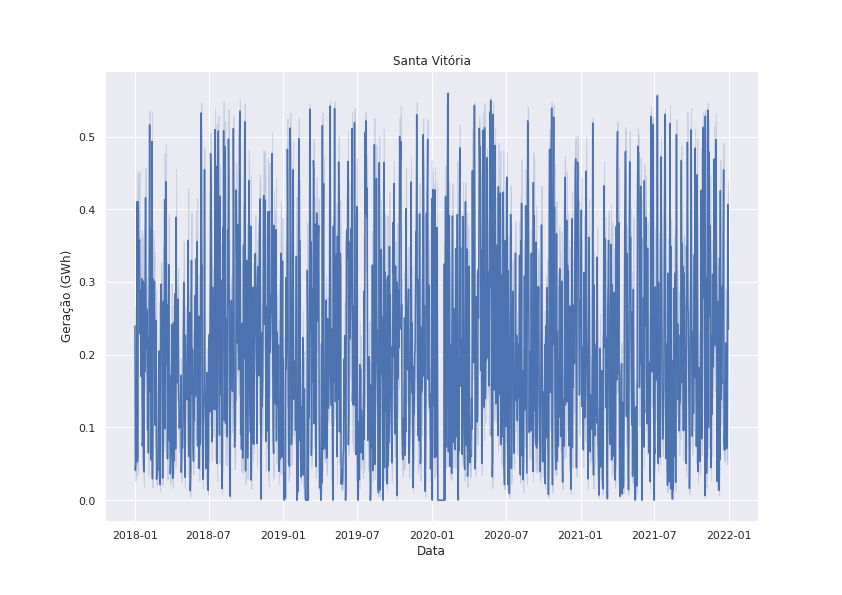
\includegraphics[width=0.5\textwidth]{Figuras/Santa_Vitoria_Historico.png}
\centering
\caption{Santa Vitória Histórico.}
\label{figura:Santa Vitória Histórico}
\end{figure}

A interpretação da distribuição dos dados nas Figuras \ref{figura:Machadinho Histórico}, \ref{figura:CMPC Histórico} e \ref{figura:Santa Vitória Histórico} pode ser melhorada por meio do uso da função de densidade de probabilidade (FDP) e a função de distribuição acumulada (FDA), conforme as figuras \ref{figura:Machadinho FDP/FDA}, \ref{figura:CMPC FDP/FDA} e \ref{figura:Santa Vitória FDP/FDA}, quais estes foram separados cada um dos dados em 10 classes (intervalos), cuja a leitura pode ser realizada no eixo y (a esquerda do gráfico), ali os dados se mostram em frequência da ocorrência, de cada classe está normalizada pelo número total de dados (35040 amostras). A apresentação do Eixo Y localizado na direita foi expressa como probabilidade de 0 a 100\%, assim apresentando esta probabilidade acumulada, assim o resultado final é 100\%, ou em números representada pela probabilidade 1.

\begin{figure}[h]
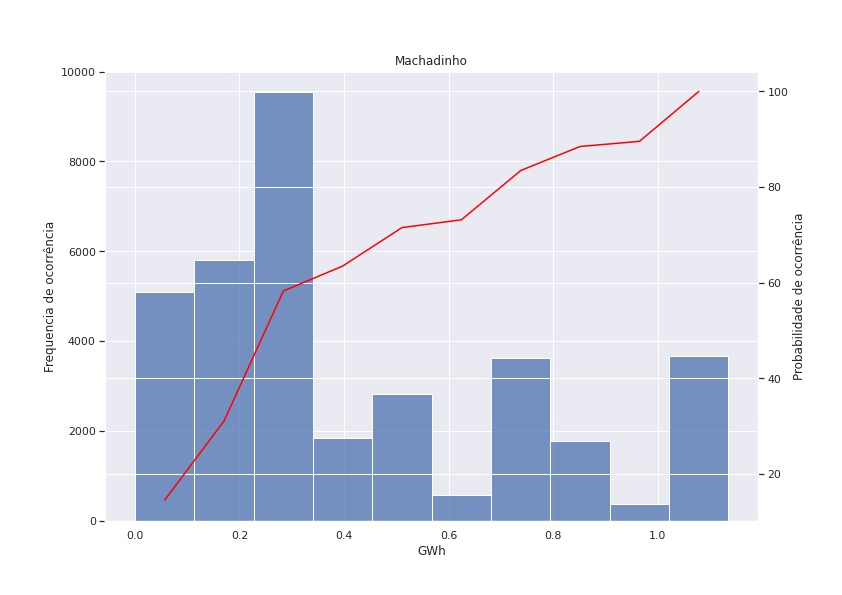
\includegraphics[width=0.5\textwidth]{Figuras/MACHADINHO.png}
\centering
\caption{Machadinho - Função de Densidade de Probabilidade e Função de Distribuição Acumulada.}
\label{figura:Machadinho FDP/FDA}
\end{figure}

\begin{figure}[h]
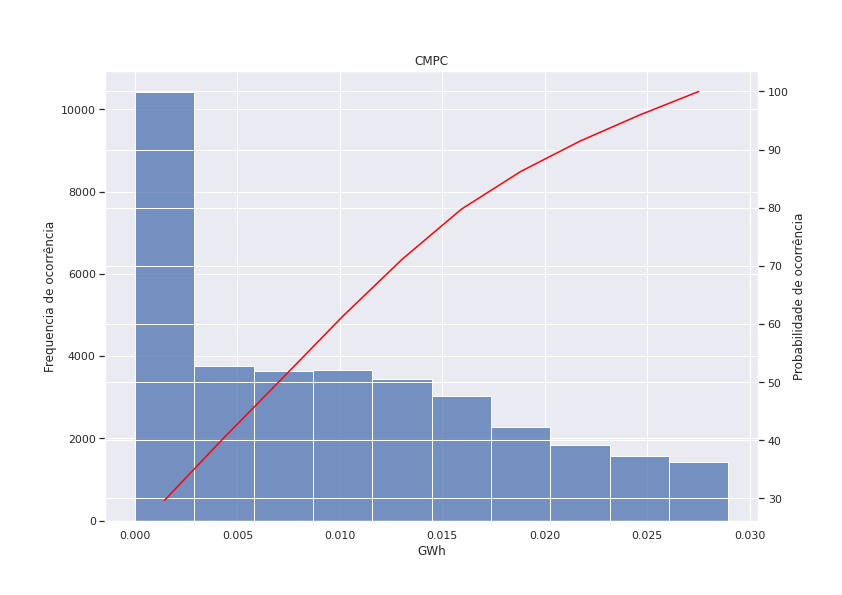
\includegraphics[width=0.5\textwidth]{Figuras/CMPC.png}
\centering
\caption{CMPC - Função de Densidade de Probabilidade e Função de Distribuição Acumulada.}
\label{figura:CMPC FDP/FDA}
\end{figure}

\begin{figure}[h]
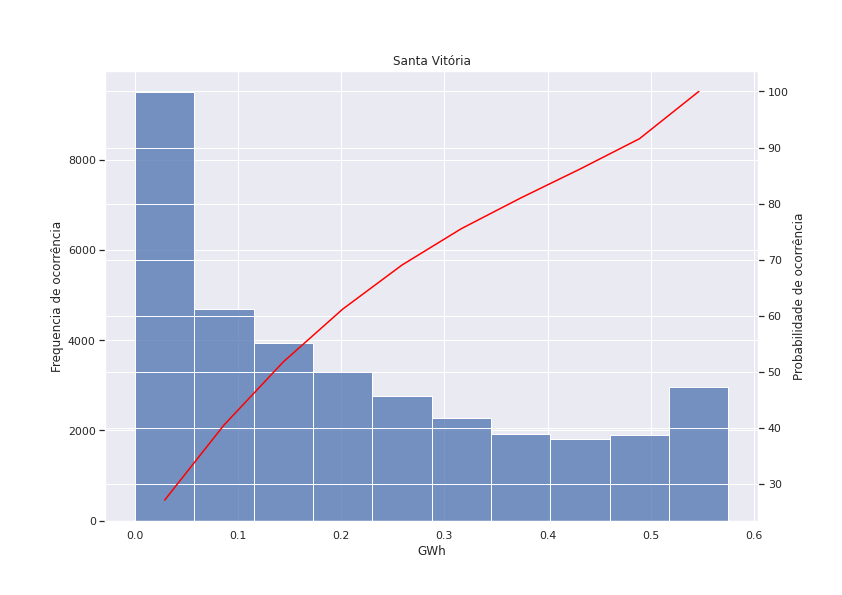
\includegraphics[width=0.5\textwidth]{Figuras/SantaVitoria.png}
\centering
\caption{Santa Vitória - Função de Densidade de Probabilidade e Função de Distribuição Acumulada..}
\label{figura:Santa Vitória FDP/FDA}
\end{figure}

Os dados utilizam métodos estatísticos, para cálculos das funções de densidade de probabilidade e função de distribuição acumulada, podemos definir que função de densidade de probabilidade (FDP) é uma equação que representa a distribuição de probabilidade de uma variável aleatória contínua e função de distribuição acumulada (FDA) é a distribuição de uma variável aleatória em uma função que nos retorna os valores somados de todas as probabilidades.

\section{Ajuste de Curvas}

Com o estudo das curvas da função de distribuição acumulada (FDA), podemos obter a curva qual pode representar o melhor a curva de probabilidade de ocorrência do valor, qual gostaríamos de obter quando temos alguns valores de geração em GWh. Assim presumi-se que a probabilidade de ocorrência está ligada a capacidade da usina.

Para este estudo de Ajuste de Curvas ou \textit{Curve Fitting em Inglês}, se utiliza de dois tipos de equações, uma equação polinomial de grau 4 (\ref{equacao:Polinomial}) e uma equação de reta (\ref{equacao:Reta}).

\begin{equation}
\label{equacao:Polinomial}
a + (b \cdot x) + (c \cdot x^{2}) + (d \cdot x^{3}) + (e \cdot x^{4})
\end{equation}

\begin{equation}
\label{equacao:Reta}
a + (b \cdot x)
\end{equation}

Quando utilizamos o \textit{fitting} polinomial (\ref{equacao:Polinomial}) para fazer o ajuste de curva de FDA disposta nas figuras \ref{figura:Machadinho FDP/FDA}, \ref{figura:CMPC FDP/FDA} e \ref{figura:Santa Vitória FDP/FDA} para achar o melhor valor de equação, dispomos de dois tipos de aproximação, para o caso de \ref{figura:Machadinho FDP/FDA}, foi utilizado a aproximação por meio da equação da reta (\ref{equacao:Reta}), assim retirando os valores com zero, fazendo uma nova equação encontramos a aproximação da curva conforme figura \ref{figura:Machadinho Fitting}.

\begin{figure}[h]
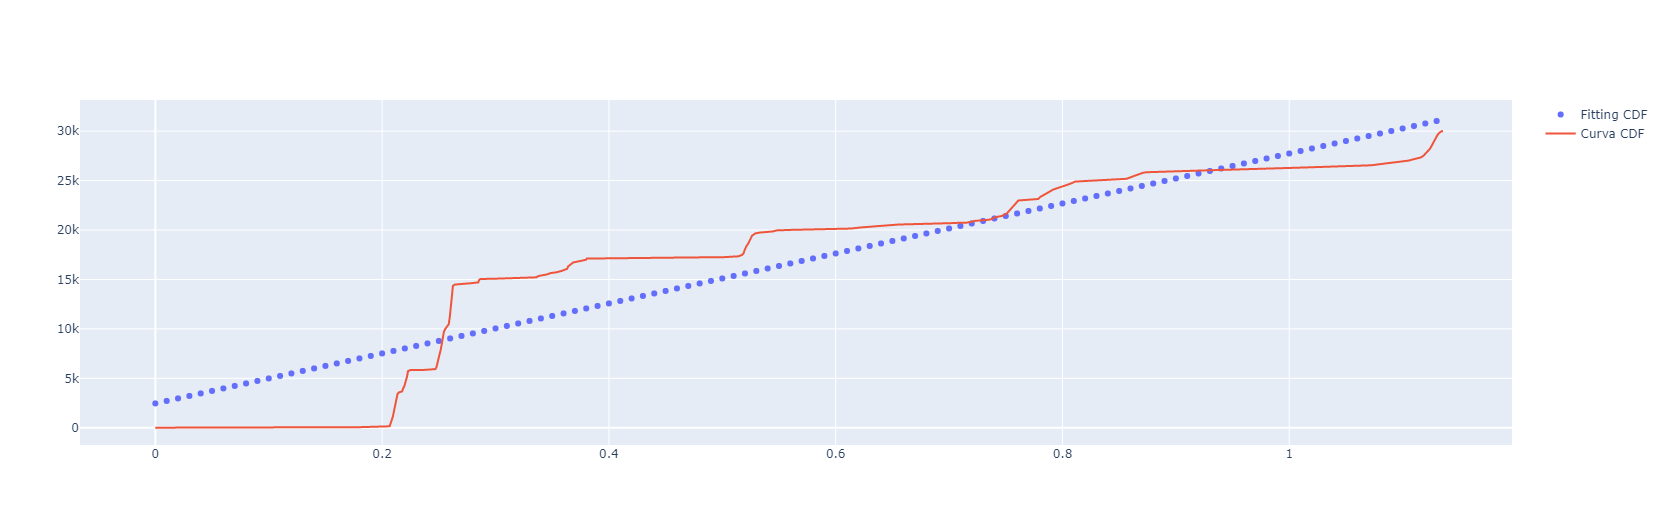
\includegraphics[width=0.50\textwidth]{Figuras/FITTING_MACHADINHO_SEM_ZERO.png}
\centering
\caption{Machadinho - Ajuste de Curvas.}
\label{figura:Machadinho Fitting}
\end{figure}

Como demonstrado na figura \ref{figura:Machadinho Fitting} o ajuste de curva não se mostra tão preciso quanto nas figuras \ref{figura:CMPC Fitting} e \ref{figura:Santa Vitoria Fitting} quais são quase curvas e a aplicação de curvas de ajuste com a equação (\ref{equacao:Polinomial}) faz um ajuste preciso conforme-os valores apresentados sem os valores nulos.

\begin{figure}[h]
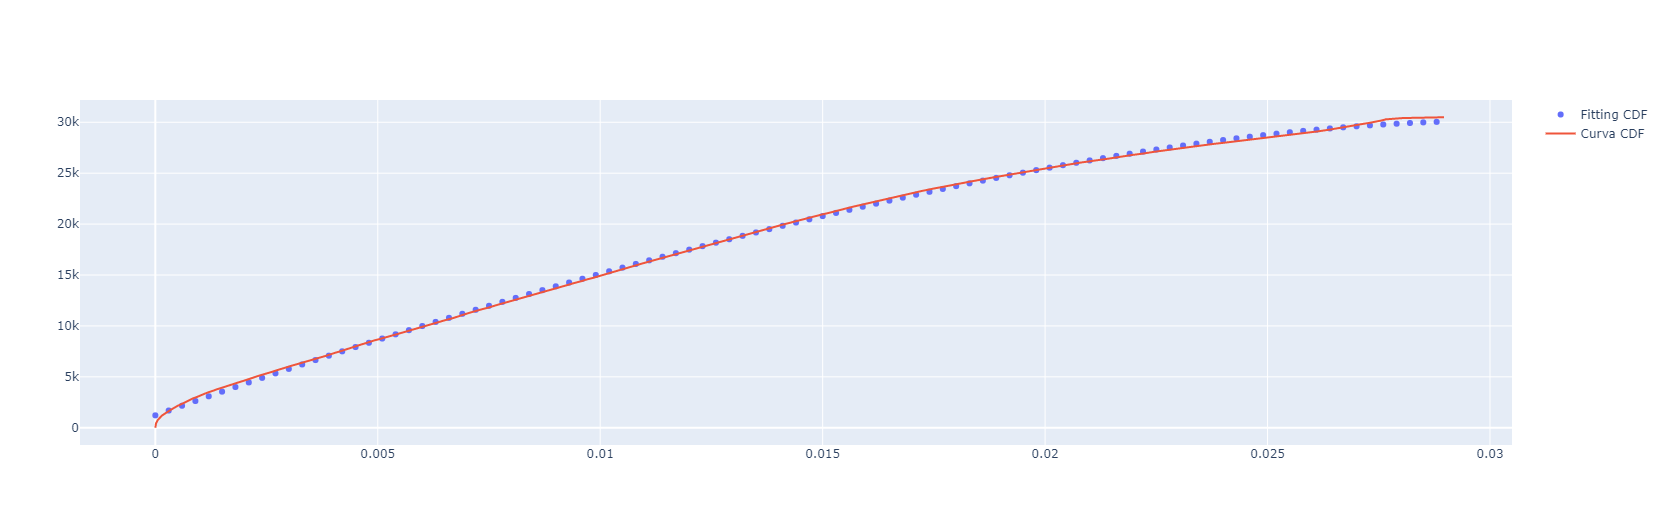
\includegraphics[width=0.5\textwidth]{Figuras/FITTING_CMPC_SEM_ZERO.png}
\centering
\caption{CMPC - Ajuste de Curvas.}
\label{figura:CMPC Fitting}
\end{figure}

\begin{figure}[h]
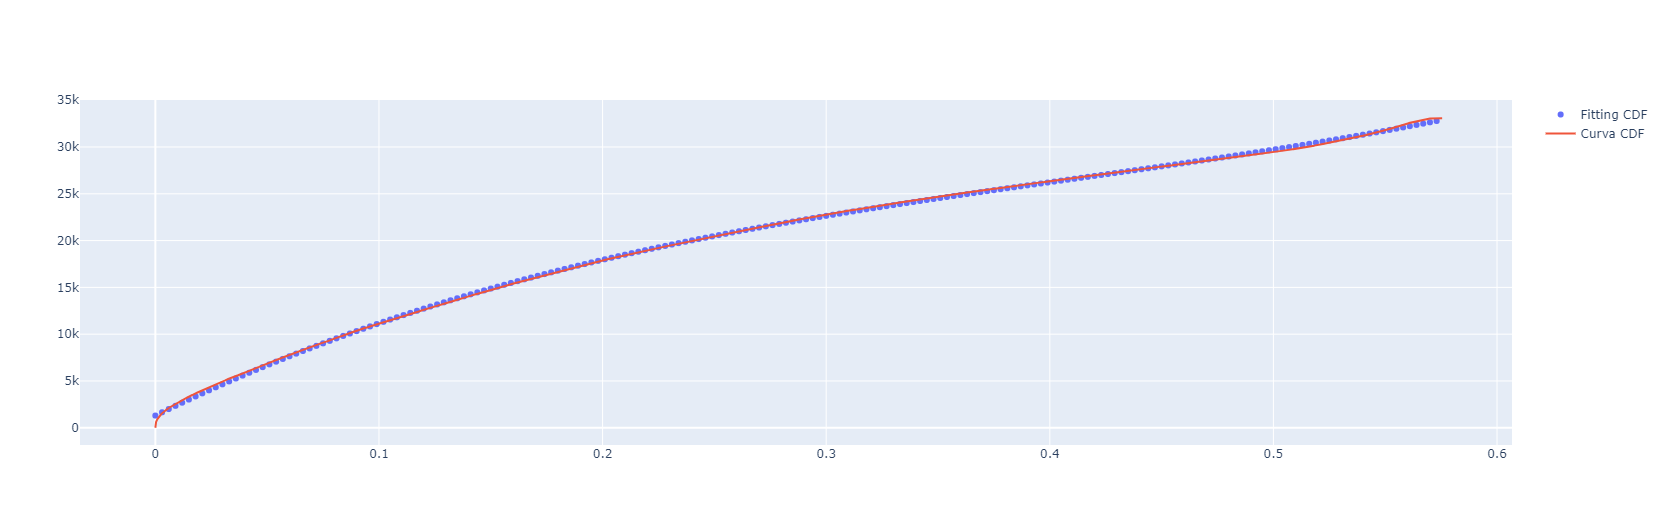
\includegraphics[width=0.5\textwidth]{Figuras/FITTING_SANTA_VITORIA_SEM_ZERO.png}
\centering
\caption{Santa Vitória - Ajuste de Curvas.}
\label{figura:Santa Vitoria Fitting}
\end{figure}

O ajuste de curvas mostrado nas figuras \ref{figura:Machadinho Fitting}, \ref{figura:CMPC Fitting} e \ref{figura:Santa Vitoria Fitting} foram feitos utilizando ferramenta \textit{"curve fit"}, disposta no pacote complementar \textit{scipy} para linguagem \textit{Python}. Todo o desenvolvimento das imagens e demais calculos foram feitos utilizando ferramentas colaborativas como o \textit{Google Colaboratory} para escrever os códigos em python e \textit{GitHub} para armazenagem dos dados em \textit{".csv"}.

Os valores para A e B em (\ref{equacao:Reta}), pode ser descrito como para a figura \ref{figura:Machadinho Fitting}:

\begin{equation}
\begin{split}
\label{equacao:Retorno Machadinho Fitting}
    a= 2461.4000\\
    b= 25276.0033
\end{split}
\end{equation}

Sendo valor em \textit{x} valor em GWh, assim substituindo (\ref{equacao:Retorno Machadinho Fitting}) em (\ref{equacao:Reta}) temos:

\begin{equation}
\label{equacao:Valor Machadinho Reta}
2461.4 + (25276.0033 \cdot x)
\end{equation}

Para os valores polinomiais de grau 4 temos os retornos em 5 componentes, sendo eles \textit{a}, \textit{b}, \textit{c}, \textit{d} e \textit{e}, assim temos o retorno dos dados de CMPC em (\ref{equacao:Retorno CMPC Fitting}) e os dados de retorno de Santa Vitória em (\ref{equacao:Retorno Santa Vitoria Fitting}).

\begin{equation}
\begin{split}
\label{equacao:Retorno CMPC Fitting}
a = 1216.2962\\
b = 1587654.6575\\
c = -23645999.3662\\
d = 540390358.7720\\
e = -14824995192.8617
\end{split}
\end{equation}

\begin{equation}
\begin{split}
\label{equacao:Retorno Santa Vitoria Fitting}
a = 1303.6236\\
b = 117120.1492\\
c = -201824.9007\\
d = 160567.4191\\
e = 3901.0616
\end{split}
\end{equation}

Sendo valor em \textit{x} valor em GWh, assim temos as seguintes equações utilizando (\ref{equacao:Retorno CMPC Fitting}) e (\ref{equacao:Retorno Santa Vitoria Fitting}) para ser substituída em (\ref{equacao:Polinomial}) assim temos:

\begin{equation}
\begin{split}
\label{equacao:Polinomial CMPC}
1216.2962 + (1587654.6575 \cdot x) + \\ (-23645999.3662 \cdot x^{2}) + (540390358.7720 \cdot x^{3}) +\\ (-14824995192.8617 \cdot x^{4})
\end{split}
\end{equation}

\begin{equation}
\begin{split}
\label{equacao:Polinomial Santa Vitoria}
1303.6236 + (117120.1492 \cdot x) + \\ (-201824.9007 \cdot x^{2}) + (160567.4191 \cdot x^{3}) +\\ (3901.0616 \cdot x^{4})
\end{split}
\end{equation}

Assim a aproximação das curvas das figuras \ref{figura:CMPC Fitting} e \ref{figura:Santa Vitoria Fitting}, utilizando as equações (\ref{equacao:Polinomial CMPC}) para usina da CMPC e (\ref{equacao:Polinomial Santa Vitoria}) e para Usina de Santa Vitória alcançamos as curvas desejadas de carga de cada usina escolhida, esse retorno se mostra preciso no caso destas duas usinas.

\subsection{Equações de Tempo}

\begin{equation}
\label{equacao:MTTF}
MTTF =\frac{1}{\lambda}
\end{equation}

\begin{equation}
\label{equacao:MTTR}
MTTR = \frac{1}{\mu}
\end{equation}

\begin{equation}
\label{equacao:MTBF}
MTBF = MTTF + MTTR
\end{equation}

\section{Considerações finais}

Atualmente a teleradiologia possui modelos que permitem essa integração de armazenamento em sua infraestrutura local, contudo, dispor de um serviço que consiga quebrar esse paradigma é bastante promissor, pois visa mostrar que a inercia presente na teleradiologia atual pode ser vencida.

Através da definição dos elementos, torna-se possível que estes atuem como gateways entre os componentes já existentes permitindo que se transponha para um serviço global sem que haja alteração no fluxo de trabalho atual, mas que permita a este fluxo ter mais dinamismo.

\addtolength{\textheight}{-12cm}   % This command serves to balance the column lengths
                                  % on the last page of the document manually. It shortens
                                  % the textheight of the last page by a suitable amount.
                                  % This command does not take effect until the next page
                                  % so it should come on the page before the last. Make
                                  % sure that you do not shorten the textheight too much.

%%%%%%%%%%%%%%%%%%%%%%%%%%%%%%%%%%%%%%%%%%%%%%%%%%%%%%%%%%%%%%%%%%%%%%%%%%%%%%%%

\bibliographystyle{IEEEtran}  
\bibliography{IEEEexample}

\end{document}
